% This is samplepaper.tex, a sample chapter demonstrating the
% LLNCS macro package for Springer Computer Science proceedings;
% Version 2.21 of 2022/01/12
%
\documentclass[runningheads]{llncs}
\pagenumbering {gobble}
%
\usepackage[T1]{fontenc}
\usepackage{hyperref}
% T1 fonts will be used to generate the final print and online PDFs,
% so please use T1 fonts in your manuscript whenever possible.
% Other font encondings may result in incorrect characters.
%
\usepackage{graphicx}
% Used for displaying a sample figure. If possible, figure files should
% be included in EPS format.
%
% If you use the hyperref package, please uncomment the following two lines
% to display URLs in blue roman font according to Springer's eBook style:
%\usepackage{color}
%\renewcommand\UrlFont{\color{blue}\rmfamily}
%
\usepackage[ngerman]{babel}

% Commands for specific words to show in italics. \Agent shows the word "Agent" in italics. 
\newcommand{\Action}{\textit{Action} }
\newcommand{\Actions}{\textit{Actions} }
\newcommand{\Agent}{\textit{Agent} }
\newcommand{\Agents}{\textit{Agents} }
\newcommand{\clear}{\textit{clear} }
\newcommand{\Dispenser}{\textit{Dispenser} }
\newcommand{\GoalZone}{\textit{Goal Zone} }
\newcommand{\GoalZones}{\textit{Goal Zones} }
\newcommand{\move}{\textit{move} }
\newcommand{\NextGroup}{\textit{NextGroup} }
\newcommand{\NextMap}{\textit{NextMap} }
\newcommand{\NextMapTile}{\textit{NextMapTile} }
\newcommand{\NextMapTiles}{\textit{NextMapTiles} }
\newcommand{\Obstacle}{\textit{Obstacle} }
\newcommand{\Obstacles}{\textit{Obstacles} }
\newcommand{\Percept}{\textit{Percept} }
\newcommand{\Percepts}{\textit{Percepts} }
\newcommand{\RoleZone}{\textit{Role Zone} }
\newcommand{\RoleZones}{\textit{Role Zones} }
\newcommand{\Step}{\textit{Step} }
\newcommand{\Steps}{\textit{Steps} }
\newcommand{\Thing}{\textit{Thing} }
\newcommand{\Things}{\textit{Things} }

\begin{document}
%
\title{Fachpraktikum Künstliche Intelligenz: Multiagentenprogrammierung}
%
%\titlerunning{Abbreviated paper title}
% If the paper title is too long for the running head, you can set
% an abbreviated paper title here
%
\author{Alexander Lorenz \and
Miriam Wolf \and
Sebastian Loder \and
Jan Steffen Jendrny}
%
\authorrunning{Lorenz A., Wolf M., Loder S., Jendrny S.}
% First names are abbreviated in the running head.
% If there are more than two authors, 'et al.' is used.
%
\institute{Fernuniversität Hagen, Universitätsstraße 47, 58097 Hagen
\url{https://www.fernuni-hagen.de/}}
%
\maketitle              % typeset the header of the contribution
%
%\begin{abstract}
%The abstract should briefly summarize the contents of the paper in
%150--250 words.
%
%\keywords{First keyword  \and Second keyword \and Another keyword.}
%\end{abstract}
%
%
%

%Einleitung
\section{Einleitung}

In diesem Kapitel wird die Auswahl der technischen Rahmenbedingungen, mit denen die Gruppe gearbeitet hat, genauer erläutert. Zudem erfolgt eine kurze Beschreibung der die Aufgaben, die von den Teammitgliedern bearbeitet wurden.

\subsection{Auswahl technischer Rahmenbedingungen}
Da die Schnittstelle der Programmierkenntnisse aller Gruppenmitglieder auf Java fiel und dies auch mit der MASSim Umgebung sowie der Vorlage des Agenten korrelierte, wurde in dieser Sprache entwickelt. Unsere Agentenvariante lief unter der Bezeichnung \textit{NextAgent}.  Alle Klassendateien beginnen mit dem Präfix \textit{Next-}, um die Zuordnung im Sourcecode zu erleichtern. Debugging erfolgte je nach Präferenz des Teilnehmers sowohl über Printausgabe in Echtzeit, als auch über Logfiles und Debugger. In kritischen Bereichen wurden Unittests umgesetzt. \\

Innerhalb des Quellcodes wurde auf Wunsch eines Teammitglieds eine spezielle Formatierung eingeführt. Dabei wurden die \textit{public} Methoden großgeschrieben, während \textit{private} Methoden weiterhin klein geschrieben wurden. Somit können öffentliche Methoden schneller erkannt und verwendet werden.

\subsection{Aufteilung Gruppenmitglieder - Arbeit}

Mit dem Ziel, den erarbeiteten Stand und weiteres Vorgehen zu besprechen, wurden wöchentliche Treffen abgehalten. Dieses konnten sehr konsequent umgesetzt werden. Initial wurde innerhalb der Gruppe versucht, in agiler Form mit Hilfe von \textit{issues} in GitHub zu arbeiten. Aufgrund der Komplexität des Themas und mangelnder Vorerfahrung der Teammitglieder, insbesondere im Kontext der Multiagentensysteme, haben wir mehr Zeit für die Einarbeitung des tieferen Verständnisses benötigt. 
\newpage
Aus diesem Grund wurden unser Konzept in vier Themenbereiche aufgeteilt, die wie folgt zugewiesen wurden:

\begin{itemize}
    \item \textbf{Herr Jendrny:} Festlegen der Aufgaben für den Agenten, basierend auf \textit{Tasks}, Normen und dem aktuellen Zustand der Welt.  
    \item \textbf{Frau Wolf:} Reaktion des Agenten auf die Umgebung und Wahl der auszuführenden \textit{Action}, mit Umsetzung der reaktiven Anteile.
    \item \textbf{Herr Lorenz:} Verarbeitung der \Percepts und Interaktion mit dem Server, optimale Wegfindung und Gruppenbildung, sowie Kommunikation.
    \item \textbf{Herr Loder:} Verarbeitung der Karte und das Zusammenführen der Karten für die Gruppe.
\end{itemize}

%Zusätzlich gab es spontan koordinierte Treffen in kleinen Teams, um Schnittstellen zu diskutieren und Lösungen für Teilbereiche zu erarbeiten. 

\subsubsection{Alexander Lorenz} ~\\
Herr Lorenz setzte die Grundvariante des Agenten um, welche die Basis für weitere Entwicklung bildete. Der Schwerpunkt lag auf der sauberen Verarbeitung der Serverdaten, der Möglichkeit zwischen den Simulationen zu wechseln und der Fähigkeit, die ersten \textit{actions} an den Server zu senden. Dabei reagierte der Agent noch rein reaktiv und wählte die nächste Aktion basierend auf einer vorgegebenen Priorisierung. \newline

Im Verlauf des Fachpraktikums setzte Herr Lorenz die Logik der Gruppenbildung um, sowie eine Variante der Kommunikation innerhalb der Gruppe. Des Weiteren beschäftigte er sich mit den Möglichkeiten zur Optimierung der Wegfindungsalgorithmen und erweiterte die initiale A* Variante, um weitere Modifikationen, die in Kapitel \textit{\ref{kap:wegfindung}} genauer beschrieben werden. Als Schnittstelle zwischen Percepts, Karte und Entscheidungsfindung wurde viel Zeit in das Bugfixing, Fehlersuche, sowie die Interpretation des Agentenverhaltens investiert. \\

Bei Herrn Lorenz lag ein Fehler in der Konfiguration der IDE, so dass Github Commits nicht sauber zugeordnet waren. Dies wurde Anfang Juni bemerkt, und behoben.  

\subsubsection{Miriam Wolf} ~\\
Um einen Schritt nach vorn zu gehen oder einen Block zu zerstören, müssen die Agenten eine \textit{Action} an den Server schicken. Um einen optimalen Weg durch die Blöcke zu finden und sich zur Endzone durchzukämpfen, muss die nächstmögliche Aktion herausgefunden werden. Frau Wolf hat sich um die Möglichkeit gekümmert, welche Aktion die nächstmögliche ist. Sie hatte die Aufgabe, das Verhalten der Agenten in der lokalen Sicht zu bearbeiten. Die Erklärung der lokalen Sicht des Agenten wird später in Kapitel \ref{kap:lokaleSicht} genauer erläutert. \\

Weiter hatte sie die Aufgabe der Praktikumsorganisatorin inne. Hierfür musste sie die Treffen der Gruppenleiter koordinieren, die Turnierplanung übernehmen und auch die Turniere begleiten. \\\\
Dazu gehörten unter anderem das Erstellen der Turnierkonfiguration oder das Starten des Servers selbst beim Turnier. Abschließend kam noch die Planung des Präsentationsnachmittags dazu und das Ausarbeiten des allgemeinen Dokumentationsteils.

\subsubsection{Sebastian Loder} ~\\
Herr Loder hat die Implementierung der Karte übernommen, welche im Detail in Kapitel \textit{\ref{erkundungDerKarte}} beschrieben ist. Die Agenten besitzen nur eine lokale Sicht, welche je \Percept abgerufen werden kann (siehe auch Kapitel \textit{\ref{kap:lokaleSicht}}). Die Informationen werden in jedem \Step übermittelt, jedoch nicht gespeichert, sodass ein Agent zunächst einmal kein Gedächtnis hat. Um zu einem späteren Zeitpunkt wieder zu bereits vorher erkundeten Bereichen zielgerichtet zurückkehren zu können, wurde die Karte implementiert, welche je Zeitschritt die lokale Sicht speichert und so die Umgebung aufnimmt. Ein wichtiger Bestandteil der Aufgabe bestand auch darin, die aufgebauten Karten der einzelnen Agenten korrekt zusammenzuführen, wenn diese sich zu einer Gruppe verbinden, siehe auch Kapitel \textit{\ref{kap:Gruppenbildung}}. \textit{Testing} und \textit{Debugging} haben in Zusammenhang mit der Karte einen relevanten Teil der Umsetzung in Anspruch genommen.

\subsubsection{Steffen Jendrny} ~\\
Herr Jendrny hat sich um die Aufgabenplanung und -verteilung unter den Agenten gekümmert. Zu Beginn der Entwicklung hat jeder Agent selbstständig entschieden, welche Aufgabe ausgewählt wird und welche Teilaufgabe momentan erfüllt werden muss. Mit der Einführung von Agentengruppen wurde die Aufgabenauswahl auf die Gruppe ausgelagert und ein Agent hat lediglich entschieden, welche Teilaufgabe momentan erfüllt werden muss. Außerdem hat Herr Jendrny zusammen mit Frau Wolf die Abgabe von Aufgaben mit mehreren Blöcken implementiert. \\
Zusammen mit Frau Wolf war Herr Jendrny bei den Lead-Treffen dabei, um Gruppe 5 zu vertreten.

%% Softwarearchitektur
\section{Softwarearchitektur}

Im ersten Unterkapitel \ref{erkundungDerKarte} wird zunächst einen Einblick in die Erkundung und die Speicherung der Karte gegeben. Hierfür wird auf die Implementierung und die Aktualisierung der Karte eingegangen, sowie auf die Veränderung in Gruppen. Ebenfalls werden die Besonderheiten der wiederholenden Karte und das Koordinatensystem erläutert. Im Kapitel \ref{kap:entscheidungAgenten} wird kurz auf die verwendeten Rollen, die Aufgaben der \textit{Agents} sowie auf die Gruppenbildung und die Wegführung eingegangen. Im Kapitel \ref{kap:lokaleSicht} wird der Unterschied zwischen lokaler und globaler Sicht des Agenten aufgezeigt. Als Abschluss in Kapitel \ref{kap:kommunikation} wird die Kommunikation der Agenten kurz erläutert.

\subsection{Erkundung und Speicherung der Karte} \label{erkundungDerKarte}

In jedem Schritt eines Spiels kann über die \Percepts abgerufen werden, welche Objekte für einen \Agent aktuell sichtbar sind. Wie weit ein \Agent sehen kann, hängt von der Rolle ab.
% Die von einem \Agent wahrgenommenen \Things werden hierbei mit relativer Distanz zur Position des \Agents angegeben. Wenn sich beispielsweise ein \Obstacle zwei Felder rechts neben dem \Agent befindet, wird dieses im \Percept mit den Koordinaten [2, 0] angegeben. Bewegt sich der \Agent anschließend um ein Feld nach rechts, wird das \Obstacle im Abstand [1, 0] gesehen. 

Informationen vergangener \Percepts sind nicht verfügbar, d.h. ein \Agent besitzt zunächst einmal kein „Gedächtnis“. Um eine zielgerichtete Planung der \Agents umzusetzen, ist es daher erforderlich, die in jedem \Step wahrgenommenen Sichten zu speichern und so Schritt-für-Schritt eine Karte aufzubauen. \\

\begin{figure}[h]
	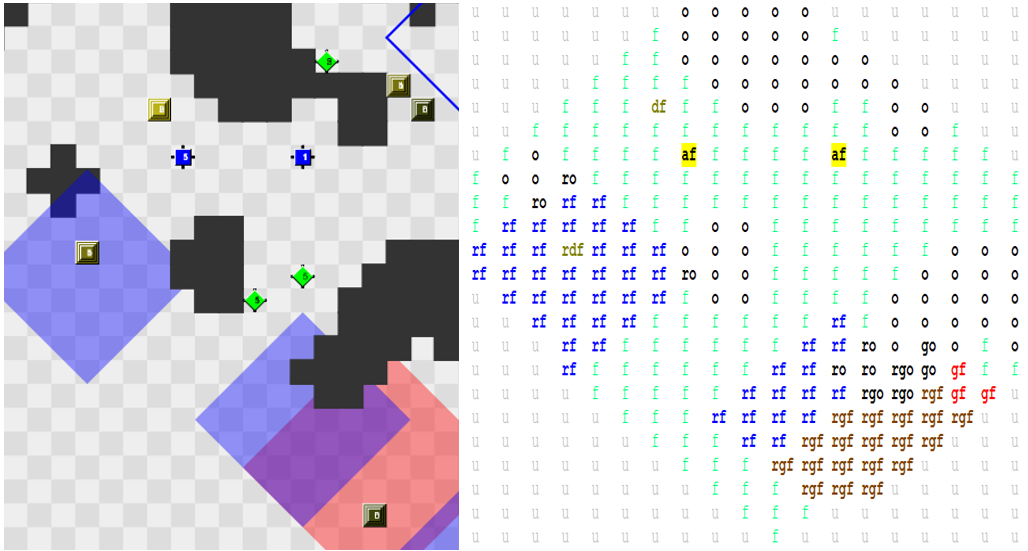
\includegraphics[width=0.7\textwidth]{./Abbildungen/map.png}
	\centering
	\label{fig:interneKarte}
	\caption{Links: Screenshot der Karte, Rechts: \NextMap-Objekt einer Gruppe mit 2 Agents als Output in eine .txt-Datei. \newline Legende: \underline{a}gent, \underline{d}ispenser, \underline{f}ree, \underline{g}oal zones, \underline{o}bstacles, \underline{r}ole zones, \underline{u}nknown}
\end{figure} 

Es ergeben sich folgende Anforderungen:
\begin{enumerate}
	\item Jeder \Agent soll die in den einzelnen \Steps wahrgenommenen \Things speichern und auf diese zu einem späteren Zeitpunkt zugreifen können. 
	\item Da manche Informationen der Karte dynamisch sind (z.B. können \Obstacles per \textit{clear()}-Befehl entfernt werden), ist auch eine Aktualisierung bereits gespeicherter Positionen erforderlich. 
	\item \Agents sollten bestenfalls dieselbe Karte verwenden, sodass jeder \Agent aus der Erkundung / aus dem Wissen der anderen \Agents schöpfen kann.
	\item Die Spiele werden mit einer sich wiederholenden Karte mit unbekannter Kartengröße gespielt. Um eine effiziente Planung zu ermöglichen, soll die Kartengröße ermittelt und die Wiederholungen bei Speicherung der Karte berücksichtigt werden.
\end{enumerate}

\newpage
\subsubsection{Aktualisierung} ~\\
Je \Agent wird geprüft, ob im letzten \Step ein erfolgreicher \move-Befehl ausgeführt wurde. Falls ja, wird die Position des \textit{Agents} aktualisiert und es werden die im \Percept übermittelten \Things zur Karte hinzugefügt bzw. bereits vorhandene Daten aktualisiert. Hierbei werden \Dispenser, \GoalZones, \RoleZones und \Obstacles gespeichert. Andere \Agents und Blöcke werden in der Karte nicht gespeichert, da sich diese meist sehr dynamisch ändern und daher in der langfristigen Wegeplanung weniger relevant sind. Abbildung \ref{fig:interneKarte} zeigt einen Vergleich der Karte des Servers mit der intern aufgebauten Karte (Export als .txt-Datei).

\subsubsection{Gruppen} ~\\
Bei Start des Spiels wird für jeden \Agent eine eigene Gruppe erzeugt, welche genau eine Karte enthält. Alle wahrgenommenen Dinge werden in dieser Karte gespeichert und sind zunächst nur für diesen \Agent sichtbar. Wenn sich zwei \Agents während des Spiels treffen, wird die Gruppe des einen Agenten mit der Gruppe des anderen Agenten zusammengeführt, siehe auch Kapitel \textit{\ref{kap:Gruppenbildung}}. In Bezug auf die Karte bedeutet dies, dass sowohl alle Agenten als auch die Kartendaten der Gruppe übertragen werden. Sofern in beiden Karten Informationen für dieselben Positionen vorhanden sind, bleibt nur das aktuellere \NextMapTile erhalten und das ältere wird verworfen. Aktualisierungen der Karte aller \Agents sind anschließend für alle anderen \Agents derselben Gruppe sichtbar. \newline

Bei den im Fachpraktikum gespielten Turnieren erfolgte die erste Zusammenführung von Gruppen meist nach nur wenigen Schritten. Innerhalb des ersten Drittel des Spiels haben die Agents i.d.R. in nur noch einer Gruppe agiert, sodass die gemeinsame Datenbasis der Karte über einen Großteil des Spiels genutzt werden konnte. 

\subsubsection{Wiederholende Karte} ~\\
Typischerweise werden die Spiele des \textit{Multi Agent Programming Contest 2022} mit einer randlosen Karte gespielt. Die Größe der Karte ist zu Beginn nicht bekannt und die Grenzen sind für die \Agents bei der Erkundung der Karte nicht erkennbar, sodass sie sich auf einer scheinbar „unendlichen“ Karte bewegen.\newline

Die Kartengröße kann herausgefunden werden, indem sich zwei \Agents treffen und anschließend in entgegengesetzte x- und y-Richtung laufen, um so die Karte „auszumessen“. Sobald sich die \Agents erneut treffen, kann durch die Anzahl der zurückgelegten Schritte die Kartengröße ermittelt werden. \\ Die Bestimmung der Kartengröße konnte leider bis zum letzten Turnier nicht mehr implementiert werden, jedoch wurde die Funktionalität der Karte bereits entsprechend vorgesehen 

Bei Bekanntwerden der Kartengröße kann diese über die allgemeine Kommunikationsschnittstelle an alle Agenten mitgeteilt werden. Anschließend werden die Positionen der \NextMapTiles und der \Agents, welche größer als die Kartengröße sind, per modulo auf die tatsächliche Kartengröße angepasst. \\
Sofern Informationen für dieselbe Position vorhanden sind, bleibt das aktuellere \NextMapTile erhalten und das ältere wird verworfen. Weitere Aktualisierungen der Karte passieren nur noch auf der tatsächlichen Kartengröße, sodass ab dem Zeitpunkt der Bekanntgabe der Kartengröße mit einer deutlichen Effizienzsteigerung zu rechnen ist. Zudem können Optimierungen bei der Wegfindung vorgenommen werden.  

\subsubsection{Globale und lokale Sicht} \label{kap:lokaleSicht}  ~\\
Bei der Sicht der \textit{Agents} kann zwischen einer globalen und lokalen Sicht unterschieden werden. Die globale Sicht besteht aus einer gespeicherten Karte pro \textit{Agent}, die sich durch die Bewegungen der \textit{Agents} auf der Karte erweitert. Hier werden die verschiedenen Dinge wie \textit{Dispenser}, \textit{Blöcke} oder Zonen gespeichert. Sobald sich die \textit{Agents} in Gruppen finden, werden die Karten synchronisiert. Eine genauere Erklärung zu den Karten befindet sich im Kapitel \textit{\ref{erkundungDerKarte}}.

\begin{figure}
	\begin{minipage}{0.6\textwidth}
		Die lokale Sicht der \textit{Agents} ist auf eine festgelegte Größe beschränkt. Die Sichtweite der \textit{Agents} wird in der Serverkonfiguration festgelegt. Bei einer Sichtweite von 5 sieht der \textit{Agent} 5 Kästchen nach links, rechts, oben und unten, wie in Abbildung \ref{fig:agentensicht} dargestellt.
	\end{minipage}
	\begin{minipage}{0.4\textwidth}
		\centering
		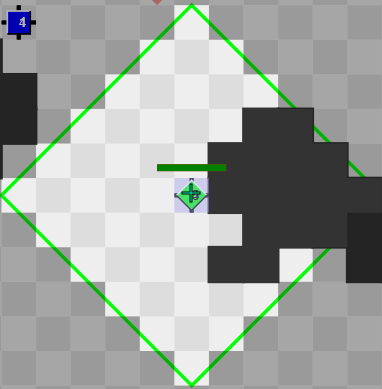
\includegraphics[width=100px]{bilder/agentensicht}
		\caption{Sicht des \textit{Agents}}
		\label{fig:agentensicht}
	\end{minipage}
\end{figure}

\subsection{Entscheidungsverhalten der Agenten} \label{kap:entscheidungAgenten}

\subsubsection{Rollen} ~\\
Während der initialen Entwicklung des \textit{Agents} wurde mit einer modifizierten \textit{default} Rolle gearbeitet, bei der alle \textit{Actions} für die Verwendung freigeschaltet waren. Ab Turnier vier wurde eine Möglichkeit eingebaut die Rollen dynamisch nach den geforderten Fähigkeiten auszuwählen. 
Somit konnte der \textit{Agent} auch auf neue, unbekannte Rollen reagieren. Allgemein wurde die Nutzung der \textit{worker}-Rolle priorisiert, die für den \textit{Agent} bis 2er \textit{task} ausreichend war. Weiterhin können die Rollen  \textit{explorer} und  \textit{digger} für die Kartenerkundung genutzt werden. Die Rolle \textit{constructor} wurde nicht eingesetzt.

\subsubsection{Aufgaben} ~\\
Um Punkte zu erzielen, müssen \textit{Agents} verschiedene Aufgaben lösen. Der Server teilt den \textit{Agents} mit, wenn es neue Aufgaben zu erledigen gibt. Die \textit{Agents} müssen Blöcke bei den \textit{Dispenser} abholen und in die Goalzones bringen.\\
Damit eine Aufgabe abgegeben werden kann, müssen die \textit{Agents} ihre Blöcke in einer bestimmten Position anordnen. Es gab Aufgaben mit einem, zwei, drei und vier Blöcken. Ab einem fixen Zeitpunkt im Spiel oder nach einer gewissen Anzahl an Abgaben, akzeptiert der Server eine Abgabe dieser Aufgabe nicht mehr. Die Abgabefrist wird den \textit{Agents} bei der Bekanntmachung einer Aufgabe mitgeteilt. Über das Erreichen des Abgabelimits bekommen die \textit{Agents} allerdings keine Information.

Zu Beginn des Praktikums wurde die Klasse \textit{NextTaskPlanner} implementiert. Da sich die Praktikumsgruppe dazu entschieden hat, dass in den ersten Turnieren nur Aufgaben mit einem Block auftreten, sollten unsere \textit{Agents} die Aufgabenplanung nicht absprechen, sondern die individuell beste Lösung finden. \textit{NextTaskPlanner} hat neue Aufgaben entgegengenommen und für alle Aufgaben eigene Pläne erstellt.
Die Pläne wurden als Baumstruktur angelegt. Die Wurzel des Baumes war die Klasse \textit{NextPlanSolveTask}. Die Zweige des Baumes waren dann jeweilige Unterpläne, repräsentiert durch verschiedene Klassen der Teilaufgaben. Die Blätter des Baumes entsprechen den auszuführenden Teilaufgaben für jeden \textit{Agents}. 
Durch eine \textit{pre-order}-Suche wird die aktuell zu erfüllende Teilaufgabe gesucht. Jeden Schritt wird durch die Wurzel des Baumes geprüft, welche Teilaufgaben bereits erledigt sin. Diese werden dann durch die Suche nicht mehr zurück gegeben.
Jeder Plan berechnet, wie viele Schritte für die Erfüllung einer Aufgabe notwendig sind. \\ \textit{NextTaskPlanner} wählt dann den Plan aus, der die meisten Punkte in Relation zu den benötigten Schritten verspricht und lässt sich dann die jeweilige Teilaufgabe ausgeben um diese dem \textit{Agents} zu übergeben.
Falls eine Aufgabe nicht erfüllt werden kann, weil entweder keine \textit{Goalzone} bekannt ist, oder die benötigten \textit{Dispenser} fehlen, erzeugt \textit{NextPlanSolveTask} die benötigten Unterpläne, um die jeweiligen Sachen auf der Karte zu finden und löscht diese Unterpläne wieder, wenn dem \textit{Agents} alle Orte bekannt sind. 

Bei späteren Turnieren wurden Aufgaben freigeschaltet, bei denen mehrere Blöcke abgegeben werden konnten. Da sich die \textit{Agents} zu einer Gruppe zusammenschließen, hat die Gruppe die weitere Planung der Aufgaben übernommen. Der Agent war allerdings weiterhin für die Auswahl der Teilpläne zuständig.
Wenn eine Aufgabe mit zwei Blocken ausgewählt wurde, dann sind zwei \textit{Agents} ausgewählt worden, um diese Aufgabe zu erfüllen. 

Die Klasse \textit{NextTaskPlanner} in der Gruppe teilte die \textit{Agents} den Aufgaben zu. Dabei wurde die Anzahl der Schritte pro verdientem Punkt minimiert und gleichzeitig verhindert, dass zu oft die gleiche Aufgabe \textit{Agents}paaren zugeordnet wurde, damit die \textit{Agents} sich auf verschiedene Dispensertypen verteilen. Die Klasse \textit{NextTaskPlanner} bestimmte auch, welcher \textit{Agent} zu welchem \textit{Dispenser} läuft. Dazu wurden in den \textit{Agents} ermittelt, wie viele Schritte benötigt werden, um den \textit{Dispenser} zu erreichen und die effizienteste Aufteilung gewählt.
Es kann ebenfalls vorkommen, dass Aufgaben mit einem Block effizienter waren oder es eine ungerade Anzahl an \textit{Agents} in einer Gruppe gab. In diesem Fall wurden den \textit{Agents} Aufgaben mit einem Block zugeordnet.

Die Entscheidung, welche Teilaufgabe zum aktuellen Zeitpunkt erfüllt werden muss, wurde dann durch die Klasse \textit{NextTaskHandler} berechnet. Dies geschah wiederum durch die oben beschriebene Baumstruktur. 

\subsubsection{Wegfindung} \label{kap:wegfindung} ~\\
Das \textit{MASSim} Szenario hat ganz besondere Anforderungen an die Wegfindungsalgorithmen. Es wird ein zweidimensionales Gitter mit 4 Nachbarn (oben, unten, links und rechts) genutzt, ohne die Diagonalen zu berücksichtigen. Die Bewegungskosten sind einheitlich, jedoch lassen sich manche Hindernisse (\textit{obstacle}, \textit{block} ) zerstören. Dies hat zur Folge, dass die Karte einem permanentem Wandel unterliegt, was Optimierungsalgorithmen, die auf Vorausberechnungen basieren, ausschließt. Der Agent verfügt innerhalb der Simulation nur die Kontrolle über einen Teil der Einheiten und muss somit immer reaktiv auf die Umgebung reagieren. \newline

Nach ersten Versuchen mit rein zufallsbasierten Bewegungsmustern, wurden das Konzept für die Planung der Bewegungen analog zur Berechnung der Manhattandistanz, sowie zur Erforschung der Karte anhand eines Spiralmusters konzipiert. Letzteres funktionierte sehr gut bei einem Agenten, erwies sich aber bei mehreren als ineffizient, da das bekannte Gebiet oft unnötig mehrmals durchlaufen wird. \\In der finalen Version wird deswegen, falls sich ein Zielpunkt außerhalb des der Karte bekannten Gebiets befindet, immer das \glqq Manhattan \grqq{} Verfahren verwendet. Ansonsten nutzt der Agent für die Berechnung des Weges den A* Algorithmus \cite{ref_proc1}. Hier wird jedoch zwischen der Planerstellung und Planausführung unterschieden. \newline

Für die Berechnung der Optionen kann man annehmen, dass das Ziel immer im bekannten Gebiet der Karte liegt. Die momentane Position der anderen \textit{Agents} und Blöcke wird ignoriert, da davon ausgegangen wird, dass diese sich zum Ausführungszeitpunkt nicht mehr an dieser Position befinden werden. Als Berechnungsoptimierung wird das \textit{A* Jump Point Search} Verfahren (A* JPS) \cite{ref_proc2} von Harabor und Grastien verwendet. Es nutzt das Konzept der Pfadsymmetrie, um die Menge der zu untersuchenden Punkte einzusparen. Dabei sind zwei Pfade dann symmetrisch, wenn sie den Start- und Endpunkt teilen und der eine aus dem anderen abgeleitet werden kann, wenn die Reihenfolge der sie bildenden Vektoren vertauscht wird. \\

Bei der Planausführung wird das klassische A* Verfahren erweitert, indem das Konzept des Wegspeichers eingeführt wird. Die Karte erfasst den geplanten Pfad, und blockiert den Weg, falls sich zu dem entsprechenden Zeitpunkt an dieser Position ein anderer Agent befindet.  Wird die Ausführung einer Bewegung durch ein Ereignis unterbrochen, wird der geplante Weg wieder freigegeben. Das Verfahren optimiert vor allem das Agieren der \textit{Agents} bei einer lokalen Anhäufung.\\
Das gleiche Problem wird auch über die lokale Neuanpassung des Pfades gelöst. Ist der nächste Schritt des \textit{Agents} blockiert, wird basierend auf den Informationen der lokalen Sicht, wie in Kapitel \textit{\ref{kap:lokaleSicht}} beschrieben, ein Teilabschnitt neu berechnet, welcher neben \textit{obstacle}, auch \textit{block} und \textit{agent} berücksichtigt. Diese Neuberechnung wird jedoch aktiv während der Wahl der nächsten Aktion getriggert. 

Als eine letzte Optimierung der Wegeberechnung wurde die Zentrierung der Karte umgesetzt. Diese erfordert zwar eine bekannte Kartengröße, durch die Möglichkeit des \textit{Agents} über den Rand zu gehen, wird aber automatisch die optimale Distanzheuristik im A* Algorithmus angewendet.



\subsubsection{Gruppenbildung} \label{kap:Gruppenbildung} ~\\
Der Ablauf der Gruppenbildung stützt sich auf den Ansatz, der von der Gruppe FitBut in \glqq{}The Multi-Agent Programming Contest 2021\grqq{} beschrieben wurde. \textit{ “If two agents see other agent at the same distance but in the opposite direction, and no other agent sees another agent at the same distance and direction, the two agents can be sure that they see each other.”}\cite{ref_book1}  \\

Für die Umsetzung wurde die durch \textit{BasicAgent}  bereitgestellte Kommunikationsplattform verwendet. Vor der Verarbeitung der \textit{Percepts}, besitzt jeder Agent den Wissenstand der letzten Runde. \\ Dieser Umstand wird genutzt, um auf den synchronen Datenstand zurückgreifen zu können. Befindet sich in der lokalen Sicht ein anderer Agent, wird eine allgemeine Nachricht mit den gesichteten Koordinaten an alle rausgeschickt. Jeder Agent prüft nun, ob sich lokal auf der gegenüber liegenden Koordinate ein Agent befindet. Diese Information wird an den ursprünglichen Sender zurück übermittelt.  

Diese Nachrichten werden gesammelt, und im nächsten Schritt ausgewertet. Sehen sich genau zwei \textit{Agents}, wird der Gruppenbildungsprozess initialisiert. Bei mehr als 2 \textit{Agents}, werden diese für diese Koordinate während der Runde gesperrt. 

\subsection{Reaktives Verhalten des Agenten}

Im ersten Schritt ermittelt der \textit{Agent} einen möglichen Weg, wie er zu seinem Ziel gelangt. Hierfür wird der entsprechende Wegalgorithmus verwendet, welcher in Kapitel \textit{\ref{kap:wegfindung}} genauer erläutert wird. Sobald der Weg ermittelt wurde und bevor ein Schritt des Weges beschritten wird, prüft der \textit{Agent} auf Aktionen, welche vorher ausgeführt werden müssen. Diese Aktionen können einen Rollenwechseln beinhalten, ungenutzte Blöcke fallen lassen, einen Block vom \textit{Dispenser} anfordern oder einen Block aufnehmen, eine Aufgabe in der Endzone abgeben oder sich mit einem anderen \textit{Agents} verbinden. Diese Aktionen sind Momentaufnahmen, die der \textit{Agent} ausführen muss, bevor er zu einem neuen Ziel geht. Wenn keine dieser Aktionen passt, wird der \textit{Agent} den Weg zu seinem Ziel gehen. Hier kommt nochmals eine Entscheidungsmöglichkeit für den \textit{Agents} in Frage. Ist der nächste Schritt frei und ich kann den Weg gehen, dann geht er diesen. Sollte aber beispielsweise ein Block in der Richtung sein, in die der \textit{Agent} gehen möchte, so muss er diesen zunächst zerstören. Wenn ein \textit{Agent} in der Richtung steht, so wird ein Weg um diesen \textit{Agents} herum erstellt. In Abbildung \ref{fig:agentensicht} wäre der Weg in Richtung Westen durch einen Block gehindert, sodass er diesen zunächst zerstören muss, bevor er in diese Richtung gehen kann. 

Zusammengefasst muss der \textit{Agent} in jedem Schritt entscheiden, ob es eine Aktion gibt, die gerade notwendig ist, wie einen Block aufzunehmen oder ob der Schritt, den er gehen möchte, möglich ist.  

\subsection{Synchronisation und Kommunikation} \label{kap:kommunikation}
Die Kommunikation der \textit{Agents} funktioniert, sobald sie sich in einer Gruppe befinden. Die Synchronisation der Gruppen ist in Kapitel \textit{\ref{kap:Gruppenbildung}} genauer beschrieben. Für die Kommunikation wurde eine Schnittstelle entwickelt, welche die Nachricht, den Senderagenten und den Empfängeragenten in einer Nachrichtenbox bereithält. Stehen zwei \textit{Agents} um einen \textit{Dispenser} und beide möchten einen Block anfordern, so wird der Agent zunächst prüfen, ob eine Nachricht für ihn vorliegt. Ist dies nicht der Fall untersucht der Agent, ob andere, zu dem Team gehörende \textit{Agents,} in der nähe des \textit{Dispenser} stehen. Wenn die Prüfung erfolgreich ist, so wird er eine Nachricht an den \textit{Agent} senden und dieser wird dann warten, bis der \textit{Dispenser} frei ist. Er selbst stellt eine Anfrage an den \textit{Dispenser} und nimmt den Block dann auf.


%% Turniere
\section{Turniere}
In diesem Kapitel wird auf die Turniere eingegangen, zudem werden die Schwierigkeiten im Turnierverlauf beschrieben.

\begin{itemize}
    \item \textbf{Turnier 1 -} 
	Das erste Turnier wurde nach einer ziemlich kurzen Entwicklungszeit abgehalten. Zu diesem Zeitpunkt waren die Agenten gerade in der Lage, die Karte zu erkunden. Der Fokus der ersten Entwicklungszeit lag auf der Kommunikation mit dem Server und sich mit den Aufgaben und den Gegebenheiten des Turniers vertraut zu machen. \newline
	
%	Das Ziel für das nächste Turnier war es, die Blöcke zu zerstören und zu den verschiedenen Zonen und Dispensern zu gehen. Eine bessere Wegfindung war ebenfalls notwendig.
	
	\item \textbf{Turnier 2 -} Beim zweiten Turnier ist der Agent die Karte mit einem spiralförmigen Weg abgelaufen und hat die Karte erkundet. Sobald er einen Dispenser in seinem Sichtfeld hatte, ging er hin und die Blöcke wurden aufgenommen. \newline

%	Für das nächste Turnier sollten die Agenten eine performante Wegfindung erhalten, die unnötigen Blöcke fallen lassen und Aufgaben klüger auswählen.
	
	\item \textbf{Turnier 3 -} Der Agent konnte Aufgaben nach Rentabilität auswählen. Das Herausfinden von Dispensern und Zonen wurde mittels der Aktion \emph{survey} umgesetzt. Der Agent konnte sich den Weg durch die \Obstacles freiräumen und den Block in die korrekte Position drehen. In das Abgeben von Tasks wurde vorher viel Zeit investiert. Durch technische Probleme mit der Verbindung zum Server am Turniertag wurden leider keine Punkte gemacht. \newline
	
	\item \textbf{Turnier 4 -} Der Agent konnte verschiedene Rollen annehmen und erfolgreich die ersten Aufgaben abgeben. Die Wegfindung erfolgte effizient und die rentabelsten Aufgaben wurden ausgewählt. Allerdings gab es noch Probleme bei einer lokalen Anhäufung von Agenten. Dies wurde vor allem deutlich, wenn sich auch die Agenten des anderen Teams um einen Dispenser oder in einer Goalzone bewegten.\newline
	
	\item \textbf{Turnier 5 -} Der Agent konnte im Ansatz 2er Tasks abgeben. Da die Turniere vorher jedoch so schlecht liefen, hat sich die Gruppe entschieden, den Agenten mit 1er Tasks zu starten. Durch die veränderte Konfiguration sind wenige 1er Tasks entstanden und die Agenten haben leider wenige Punkte gemacht. \newline
%	Es wurde ein Problem bei der Kartierung beobachtet.
	
	\item \textbf{Turnier 6 -} 	Die Umsetzung der 2er Tasks war stabil, die Agenten konnten miteinander kommunizieren und sich miteinander verbinden. Die Umschaltung zwischen 1er und 2er Tasks hat sehr gut funktioniert und die Agenten haben sich auch nur selten gegenseitig blockiert, so dass das Team einige Punkte holen konnte. \newline

\end{itemize}

\subsection{Schwierigkeiten im Turnierverlauf}
Bei der Karte setzten wir vom Beginn der Entwicklung auf eine randlose Karte. Dies führte zu einigen Problemen, die auch unsere Performance in den Turnieren stark beeinträchtigten. Die \Agents wanderten nach links oben und haben dadurch die Größe der Karte massiv gestreckt, wie in Abbildung \ref{fig:kartenwiederholung} dargestellt. Dies führte zu sehr vielen redundanten Bewegungen und kostete leider unnötig Zeit.  \newline

In unseren Versuchen setzten wir auf spezialisierte Umgebungen, um Teilbereiche zu optimieren. Hier trat das Verhalten nur selten auf und wurde dadurch kaum beobachtet. In der Turnierumgebung wurde es jedoch sehr dominant, und spätestens im fünften Turnier wurde dieses Verhalten als extrem kritisch eingestuft und konnte beseitigt werden. Bis zum vierten Turnier hatten wir zusätzlich Probleme mit der Synchronisierung der Karte, welche durch dieses Verhalten verschärft wurden. \newline

%Durch die Organisationsrolle von Frau Wolf konnte die Gruppe leider nicht auf das volle Potential eines erfahrenen Entwicklers zuruckgreifen.

%Das nächste Problem, welches das Team zu bewältigen hatte war die Auswahl der Tasks nach Profitabilität und die Gruppenbildung, damit die \Agents im Team die Aufgaben lösen können. 


\begin{figure}
	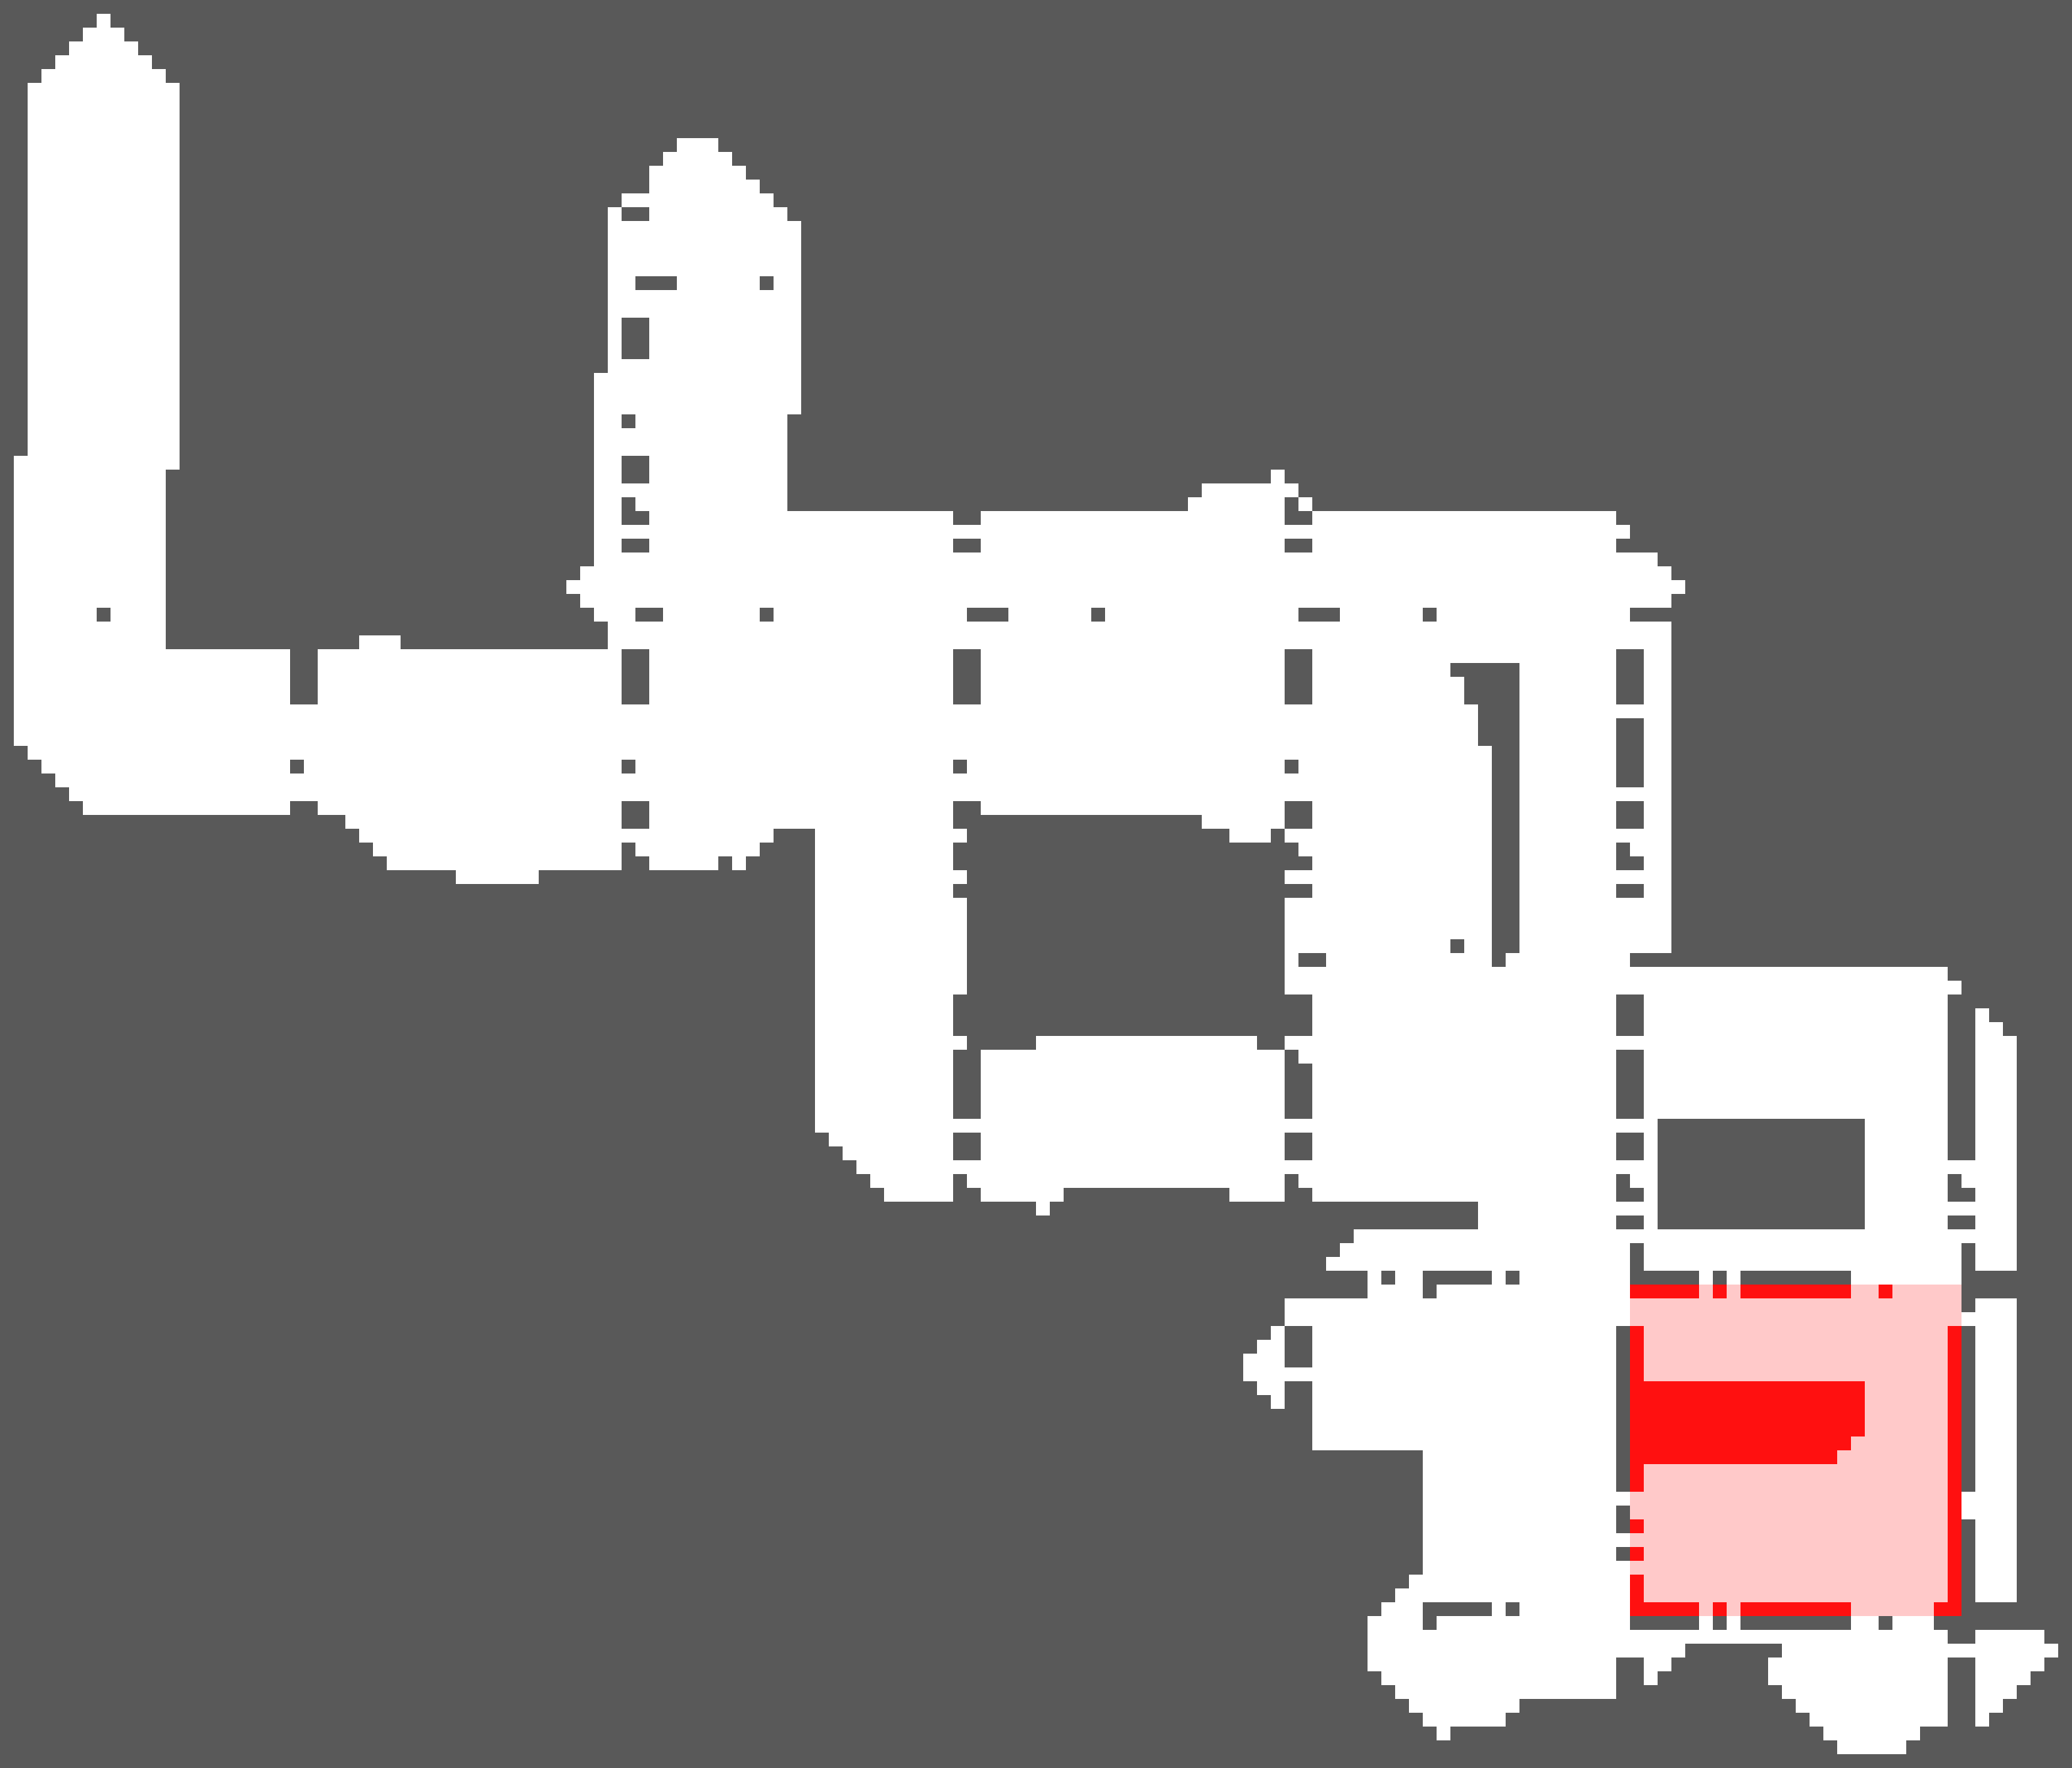
\includegraphics[width=180px]{bilder/karte3.png}
	\centering
	\caption{Beispiel für eine gestreckte Karte basierend auf einer 24x24 Welt }
	\label{fig:kartenwiederholung}
\end{figure}


%\subsection{Lösungsstrategien}
%Die Lösungsstrategien werden zu den Themenbereichen aufgeteilt und kurz erläutert:

%\begin{itemize}

%	\item \textbf{Wegfindung -} 	Zu Beginn sind die \Agents zufällig über die Karte gelaufen. Als einfachen Wegfindung wurde dann ein Spiralförmiger Weg gewählt, um die Karte zu erkunden und zufällig passende \Dispenser zu finden. Die Entwicklung des A* begann ziemlich früh und wurde die meiste Zeit des Praktikums optimiert und weiterentwickelt. 	\newline
	
%	\item \textbf{Kommunikation -} Die Kommunikation unter den \Agents wurde bei uns nur in der Gruppe umgesetzt. Da die Agenten meistens in der Mitte des Spiels zu einer Gruppe gefunden haben, hat es uns nicht eingeschränkt. Hierfür wurde eine Art Nachrichtenbox erstellt, aus der die \Agents Nachrichten auslesen oder hineinlegen konnten. Auch das Problem mit dem gegenseitigen Blockieren konnte mittels der Kommunikation gelöst werden 	\newline

%	\item \textbf{Karte -} Während des Suchens der verschiedenen Ziele wurde unsere Karte immer nach links oben erweitert. Dies war ein simpler Fehler, der die Gruppe einige Wochen gekostet hat. Dabei hat sich beim zufälligen Suchen ein Fehler eingeschlichen, der die Agenten immer in eine Richtung hat gehen lassen. Nachdem der Fehler behoben war, blieb die Karte kleiner und der Wegfindealgorithmus hat noch besser funktioniert.

%\end{itemize}

%\subsection{Interaktion mit/gegen andere Agenten}
%Die anderen Agenten wurden primär als Fremdkörper interpretiert, denen ausgewichen werden konnte, jedoch wurde keine aktive Interaktion mit diesen angestrebt. Ein Ansatz, statt den Agenten die Blöcke anzugreifen, wurde durch das MASSim Regelwerk verhindert. 

%% Fazit
\section{Fazit}

\subsection{Schwierigkeiten}

Bei der Karte setzten wir vom Beginn der Entwicklung auf eine randlose Karte. Dies führte zu einigen Problemen, die auch unsere Performance in den Turnieren stark beeinträchtigten. Z.B. trat ein Fehler im Verhalten zu einem bestimmten Zeitpunkt auf, welcher zuerst als gewolltes Feature fehlinterpretiert wurde. Die Agenten wanderten nach links oben, und haben dadurch die Größe der Karte massiv gestreckt, wie in Abbildung \ref{fig:kartenwiederholung} dargestellt. Dies führte zu sehr vielen redundanten Bewegungen, und kostete leider unnötig Zeit. \\

\begin{figure}
    \includegraphics[width=150px]{bilder/karte.png}
    \centering
    \caption{Beispiel für eine gestreckte Karte basierend auf einer 24x24 Welt }
    \label{fig:kartenwiederholung}
\end{figure}

In unseren Versuchen setzten wir auf spezialisierte Umgebungen, um Teilbereiche zu optimieren. Hier trat das Verhalten nur selten auf, und wurde dadurch kaum beobachtet. In der Turnierumgebung wurde es jedoch sehr dominant, und spätestens im Turnier5 wurde dieses Verhalten als extrem kritisch eingestuft, und konnte beseitigt werden. Bis zum Turnier4 hatten wir noch Probleme mit der Synchronisierung der Karte, welche durch dieses Verhalten verschärft wurden. \\

%Um die Fehler endgültig zu beseitigen, wurde zusätzlich ein Verfahren entwickelt, um die Karte zu vermessen. Dieses konnte leider nur teilweise umgesetzt werden. 

\subsection{Ausblick und weitere Möglichkeiten}

%% FAQ
%\section{FAQ Gruppe 5}

\subsection{Teilnehmer*innen und ihr Hintergrund}
\subsubsection{Was war die Motivation an dem Praktikum teilzunehmen?}
\subsubsection{Wurden die Agents von Grund auf neu implementiert oder auf einer bestehenden Lösung aufgebaut?}
Die Agents basieren auf der Klasse \textit{Agent} der MASSim 2022-Implementierung, wurde ansonsten komplett selbst entwickelt.
\subsubsection{Wie viel Zeit wurde in die Entwicklung und Organisation des Praktikums gesteckt?}
Die meiste Zeit wurde in die Entwicklung der Agenten gesteckt. Circa 6 Stunden pro Person pro Woche (April - September) sind in die Entwicklung und Organisation geflossen. Insgesamt schätzen wir den Umfang auf über 600 Stunden.
\subsubsection{Wie war die reingesteckte Zeit im Verlauf des Praktikums verteilt?}
Zu Beginn der Praktikums wurde viel Zeit in die Organisation und die Theorie gesteckt. Bereits nach wenigen Wochen startete die Entwicklung, die sich bis zum Ende des Praktikums gleichmäßig fortgesetzt hat. Wöchentlich gab es ein Treffen, um den aktuellen Stand zu besprechen.
\subsubsection{Wie viele Zeilen Code wurden ungefähr geschrieben?}
\subsubsection{Welche Programmiersprache und Entwicklungsumgebung wurde verwendet?}
Es wurde in Java 17 entwickelt und es kamen verschiedene Entwicklungsumgebungen zum Einsatz (IntelliJ IDEA, Netbeans, Eclipse)
\subsubsection{Wurden externe Werkzeuge/Bibliotheken verwendet?}
Nein, außer der Entwicklungsumgebung und der MASSim 2022 implementierung gab es keine Werkzeuge.
\subsection{Agenten-System Details}
\subsubsection{Wie entscheiden die Agenten, was sie machen sollen?}
Die Agenten schließen sich in Gruppen zusammen, die die Aufgaben an die Agenten verteilt. Welche Teilaufgaben die Agenten momentan erfüllen müssen, entscheidet jeder Agent selbstständig.
\subsubsection{Wie entscheiden die Agenten, wie sie etwas machen sollen?}
Die Agenten berechnen den Weg zu einem Ziel anhand einer gruppenweit geteilten Karte. Anhand der Sicht eines Agenten, entscheidet sich der Agent für den nächsten Schritt.
\subsubsection{Wie arbeiten die Agenten zusammen und wie dezentralisiert ist der Ansatz?}
Alle Agenten befinden sich in einer Gruppe. Wenn sich zwei Agenten treffen, werden diese Gruppen fusioniert. Im optimalen Fall, befinden sich nach einer Weile alle Agenten in der selben Gruppe. Dort werden die Agenten zu paaren zusammengestellt und können so gemeinsam Aufgaben lösen. Das konkrete Verhalten wird jedoch dezentral vom Agenten gelöst.
\subsubsection{Kann ein Agent das generelle Verhalten zur Laufzeit ändern?}
Ja, der Agent kann das Verhalten zur Laufzeit ändern. Dies kommt zum Beispiel vor, wenn Goalzones die Position auf der Karte verändern.
\subsubsection{Wurden Änderungen (z.B kritische Fehler) während eines Turniers vorgenommen?}
Während eines Turniers wurden keine Fehler behoben. Bei einem Turnier gab es zwar Probleme, die lagen jedoch an einem Hintergrundprozess, der die Kommunikation mit dem Server behinderte.
Auf programmatischer Seite, gab es lediglich einen spontanen Versuch im letzten Turnier das gegnerische Team zu stören, das während einer Spielpause kurz implementiert wurde.
\subsubsection{Wurde Zeit investiert um die Agenten fehlertoleranter zu machen? Wenn ja, wie genau?}
Es wurde viel Zeit genutzt, damit die Agenten fehlertolerant Agieren. Eine Person hat sich hauptsächlich mit diesem Thema beschäftigt. Es wurden sehr viele Fallunterscheidungen implementiert.
\subsection{Szenario und Strategie}
\subsubsection{Was ist die Hauptstrategie der Agenten?}
Die Agenten versuchen mit möglichst wenig Schritten möglichst viele Punkte zu erzielen. Dazu berechnen sie die optimale Aufgabe und versuchen diese zu lösen. Wenn Aufgaben mit zwei oder mehr Blöcken die optimale ist, dann werden die Agenten zu festen Gruppen zusammengefügt.
\subsubsection{Haben die Agenten selbstständig eine Strategie entwickelt oder wurde diese bereits in die Implementierung eingebaut?}
Die Strategie ist fest implementiert.
\subsubsection{Wurde eine Strategie implementiert, die Agenten anderer Teams mit einbezieht?}
Nein, die Agenten anderer Teams wurden nicht in die Strategie mit aufgenommen.
\subsubsection{Wie entscheiden Agenten, welche Aufgabe sie als nächstes übernehmen?}
Die Gruppe berechnet die optimale Aufgabe und teilt diese den Agenten mit.
\subsubsection{Wie koordinieren die Agenten die Arbeit für eine Aufgabe untereinander?}
Die Gruppe übernimmt die Koordination. Sie fragt, wo die Agenten stehen und bestimmt dann die beste Verteilung. Die Agenten holen dann selbstständig die Blöcke ab, bringen sie zur Goalzone, warten auf den Partner, verbinden sich mit diesem und geben die Aufgabe ab.
\subsubsection{Welche Aspekte des Szenarios waren am Herausforderndsten?}
Die Aufgaben mit mehreren Blöcken haben in der Entwicklung sehr große Probleme hervorgerufen.
\subsection{Und die Moral von der Geschichte}
\subsubsection{Was wurde durch das Praktikum vermittelt?}
Die Multiagentenprogrammierung und viele Hindernisse in diesem Themenfeld konnten vermittelt werden. Es wurde diskutiert, welche Strategie und Architektur sinnvoll sind und es wurde geforscht, wie die Kommunikation, Fehlertoleranz und die Strategie am besten funktioniert.
\subsubsection{Welchen Ratschlag wäre für zukünftige Gruppen sinnvoll?}
Sehr früh damit beginnen die Agenten flexibel und Fehlertolerant zu gestalten.
\subsubsection{Was waren Stärken und Schwächen der Gruppe?}
Zu Beginn haben wir Probleme in der Gruppenorganisation gehabt, die die Absprache schwierig gemacht haben. Eine große stärke der Gruppe war allerdings, dass wir mit einer enormen Konstanz, Spontanität Offenheit an diesem Praktikum gearbeitet haben. Dadurch konnten Probleme schnell gelöst werden und das Klima lange positiv gehalten werden.
\subsubsection{Was waren Vorteile und Nachteile der gewählten Programmiersprache und weiterer Werkzeuge?}
Java hatte den sehr großen Vorteil, dass die MASSim 2022 Implementierung bereits in Java geschrieben war und uns dadurch viel Arbeit erspart geblieben ist.
\subsubsection{Welche weiteren Probleme und Herausforderungen kamen im Laufe des Praktikums auf?}
\subsubsection{Was könnte beim nächsten Praktikum verbessert werden?}
Es könnte ein festes Ziel geben, auf das Hingearbeitet werden kann, dadurch kann der Arbeitsaufwand reduziert werden und eine genauere Planung der Arbeitsschritte wäre möglich.
\subsubsection{Welcher Aspekt der Gruppenarbeit hat am meisten Zeit in Anspruch genommen?}
Die meiste Zeit wurde in die Absprachen der Aufgaben investiert.

%
% ---- Bibliography ----
%
% BibTeX users should specify bibliography style 'splncs04'.
% References will then be sorted and formatted in the correct style.
%
% \bibliographystyle{splncs04}
% \bibliography{mybibliography}
%

\begin{thebibliography}{8}
	\bibitem{eclipse} https://www.eclipse.org/
	\bibitem{intellij} https://www.jetbrains.com/idea/
	\bibitem{netbeans} https://netbeans.apache.org/
	\bibitem{ref_book1} Ahlbrecht Tobias, Dix Jürgen, Fiekas Niklas, Krausburg Tabajara: The Multi-Agent Programming Contest 2021. One-and-a-Half Decades of Exploring Multi-Agent Systems, pp. 27. Springer Nature, Singapore(2021)
	
	
	%Beispiele Am ENde zum löschen
	%\bibitem{ref_lncs1}
	%Author, F., Author, S.: Title of a proceedings paper. In: Editor,
	%F., Editor, S. (eds.) CONFERENCE 2016, LNCS, vol. 9999, pp. 1--13.
	%Springer, Heidelberg (2016). \doi{10.10007/1234567890}
	%
	%\bibitem{ref_book1}
	%Author, F., Author, S., Author, T.: Book title. 2nd edn. Publisher,
	%Location (1999)
	%
	%\bibitem{ref_proc1}
	%Author, A.-B.: Contribution title. In: 9th International Proceedings
	%on Proceedings, pp. 1--2. Publisher, Location (2010)
	%
	%\bibitem{ref_url1}
	%LNCS Homepage, \url{http://www.springer.com/lncs}. Last accessed 4
	%Oct 2017
\end{thebibliography}

\end{document}
